\documentclass[11pt,letterpaper]{article}
\usepackage{fontspec}
\setmainfont{texgyrepagella}[Extension=.otf,UprightFont=*-regular,BoldFont=*-bold,ItalicFont=*-italic,BoldItalicFont=*-bolditalic]
\usepackage[bidi=default]{babel}
\babelprovide[import,main]{spanish}
\babelprovide[import]{hebrew}
\babelprovide[import]{ancientgreek}
\babelfont[hebrew]{rm}[Path=fonts/,BoldFont=NotoHebrewSerif-700.ttf,Scale=0.95]{NotoHebrewSerif-400.ttf}
\babelfont[ancientgreek]{rm}[Path=fonts/]{GFSPorson.otf}
\newcommand{\heb}[1]{\mbox{\foreignlanguage{hebrew}{#1}}}
\newcommand{\grc}[1]{\foreignlanguage{ancientgreek}{#1}}
\usepackage{needspace}
\newcommand{\hebverso}[1]{\par\needspace{7\baselineskip}\smallskip{\centering\begin{otherlanguage}{hebrew}\large #1\end{otherlanguage}\par}\smallskip}
\usepackage[margin=2.5cm,headheight=14pt]{geometry}
\usepackage{microtype,ragged2e,booktabs,graphicx,xcolor,csquotes,array}
\usepackage[hidelinks]{hyperref}\usepackage{xurl}\urlstyle{same}
\usepackage[most]{tcolorbox}
\usepackage{tikz}\usetikzlibrary{arrows.meta,positioning,calc,decorations.pathreplacing}
\usepackage{titlesec,fancyhdr,extramarks}
% Paleta "Israel": celeste y azul del tejelet (Nm 15:38) con oro del santuario
% (nombres conservados por compatibilidad: ladrillo = azul tejelet, cafe = azul real, cafeosc = azul noche,
%  piedra = celeste claro, sepia = azul pizarra)
\definecolor{cafe}{RGB}{26,82,150}\definecolor{cafeosc}{RGB}{11,33,74}\definecolor{tinta}{RGB}{20,32,56}
\definecolor{oro}{RGB}{206,162,52}\definecolor{ladrillo}{RGB}{20,68,140}
\definecolor{piedra}{RGB}{234,243,251}\definecolor{sepia}{RGB}{72,102,140}\definecolor{celeste}{RGB}{96,166,222}
\titleformat{\section}{\Large\bfseries\color{ladrillo}}{\thesection.}{0.6em}{}
\titleformat{\subsection}{\large\bfseries\color{cafe}}{\thesubsection}{0.6em}{}
\pagestyle{fancy}\fancyhf{}
\fancyhead[L]{\foreignlanguage{spanish}{\small\itshape\color{sepia}\firstleftmark}}\fancyhead[R]{\foreignlanguage{spanish}{\small\color{sepia}\thepage}}
\renewcommand{\sectionmark}[1]{\markboth{#1}{}}
\setlength{\parindent}{1.27cm}\linespread{1.15}\setlength{\emergencystretch}{3em}
\newtcolorbox{cita}[1][]{enhanced,colback=piedra,colframe=oro!90!ladrillo,boxrule=0pt,leftrule=2.5pt,arc=0pt,
  left=8pt,right=8pt,top=5pt,bottom=5pt,before skip=8pt,after skip=8pt,fontupper=\itshape,#1}
\newcommand{\fuente}[1]{\par\hfill{\upshape\bfseries\small\textcolor{ladrillo}{#1}}}
\newtcolorbox{nota}[1][]{enhanced,colback=oro!12,colframe=oro!80!ladrillo,boxrule=0.6pt,arc=2pt,
  fonttitle=\bfseries\small,coltitle=cafe,colbacktitle=oro!35,fontupper=\small,title={#1}}
\newcommand{\refapa}[1]{\par{\RaggedRight\hangindent=1.27cm\hangafter=1\noindent #1\par}\vspace{4pt}}
\newcommand{\destacar}[1]{\textbf{\textcolor{ladrillo}{#1}}}
\title{\color{ladrillo}\bfseries Del Éxodo a la muerte de Josué\\[4pt]\large\color{cafe}\mdseries Un pueblo redimido para ser reino de sacerdotes, sostenido por la misericordia que perdona y conducido a la tierra prometida}
\author{}\date{\color{sepia}Serie «Israel, el pueblo de Dios» · Estudio 2}
\begin{document}
\maketitle\thispagestyle{empty}

\begin{abstract}\noindent
Este segundo estudio recorre la historia de Israel desde la Pascua en Egipto hasta la muerte de Josué, y muestra que la Torá ya anuncia en esta etapa la restauración de Israel, porque el pacto roto al pie del Sinaí se renueva sobre el nombre misericordioso de Dios y Moisés predice, antes de entrar en la tierra, el destierro y el regreso. Sigue el relato desde la vocación de «reino de sacerdotes y nación santa» (Éx 19:6) hasta la asamblea de Siquem, y lee sus rupturas a la luz de la intercesión de Moisés, del remanente de Josué y Caleb y de Dt 4:25–31 y 30:1–10. Expone los hallazgos arqueológicos del período con sus debates, recoge la memoria judía de Shavuot, las trece midot y el 9 de Av, y sigue a Isaías, Jeremías y Oseas, que anuncian un nuevo éxodo y un nuevo pacto, hasta Romanos 9–11, donde Pablo funda su esperanza para Israel en textos de Deuteronomio.
\par\smallskip\noindent\textbf{Palabras clave:} Éxodo, Sinaí, reino de sacerdotes, tabernáculo, Deuteronomio, Josué, nuevo pacto, Romanos 11.
\end{abstract}

\section{Introducción}

Salir de Egipto no bastaba para que un grupo de esclavos liberados llegara a ser un pueblo. Tres meses después del paso del mar, Dios conduce a Israel al Sinaí y le revela para qué lo ha sacado: «vosotros me seréis un reino de sacerdotes y una nación santa» (Éx 19:6). La redención tenía un destino, y ese destino era una tarea ante las naciones. No sorprende que Pablo, al enumerar los dones irrevocables de Israel, nombre justamente los que nacen en esta etapa: «la gloria, los pactos, la promulgación de la ley, el culto» (Ro 9:4).

El mismo período que da forma a esa vocación registra también su primera quiebra. Cuarenta días después de prometer obediencia, Israel adora un becerro de oro; en Cades quiere volver a Egipto, y en Baal-peor se entrega a los cultos de Moab. A cada ruptura responde, sin embargo, una palabra de restauración. Dios se da a conocer como «compasivo y clemente» (Éx 34:6) inmediatamente después del becerro, perdona en Cades mientras preserva un remanente, y en las llanuras de Moab, antes de que Israel pise la tierra, Moisés le anuncia que la perderá y que volverá a ella (Dt 4:25–31; 30:1–10). Sobre esos textos, los más explícitos de toda la Torá, construirán Isaías, Jeremías y Oseas el anuncio de un nuevo éxodo y un nuevo pacto, y Pablo la esperanza de Romanos 11.

\begin{nota}[Sobre traducción, numeración y fechas]
Traducción propia desde el hebreo (BHS) y el griego (NA28); la LXX según Rahlfs-Hanhart. Si la numeración hebrea difiere, va entre corchetes: Dt 29:4 [29:3]. Fechas: a.\,e.\,c. (antes de la era común) y e.\,c.
\end{nota}

\section{Marco cronológico}

El relato ofrece una cronología interna muy precisa para el primer y el último año del desierto. Israel sale de Egipto el día 15 del primer mes (Nm 33:3), llega al Sinaí «al tercer mes» (Éx 19:1) y levanta el tabernáculo el primer día del segundo año (Éx 40:17). Tras Cades vienen cuarenta años de desierto, «un año por cada día» de la exploración (Nm 14:34). Moisés pronuncia Deuteronomio en el undécimo mes del año cuarenta (Dt 1:3), e Israel cruza el Jordán el día 10 del primer mes (Jos 4:19), la fecha en que Éx 12:3 manda separar el cordero.

\begin{center}
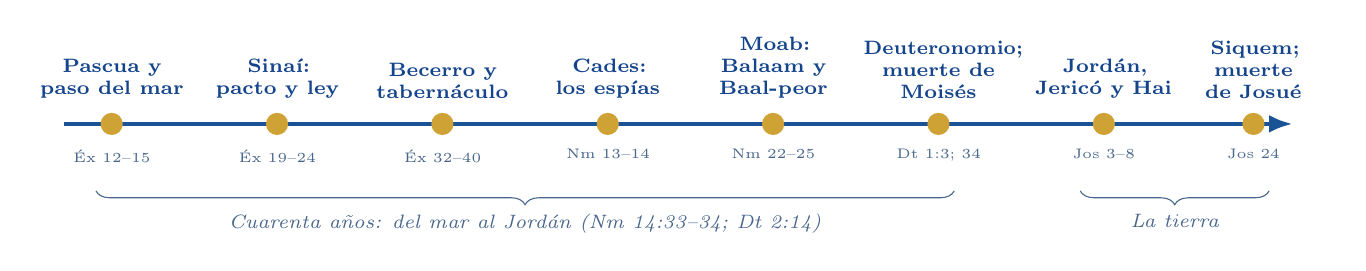
\begin{tikzpicture}[x=1cm,y=1cm]
\draw[line width=1.6pt,cafe,-{Latex[length=3mm]}] (0,0) -- (15.6,0);
\foreach \x/\t/\b in {0.6/{Pascua y paso del mar}/{Éx 12--15},
                      2.7/{Sinaí: pacto y ley}/{Éx 19--24},
                      4.8/{Becerro y tabernáculo}/{Éx 32--40},
                      6.9/{Cades: los espías}/{Nm 13--14},
                      9.0/{Moab: Balaam y Baal-peor}/{Nm 22--25},
                      11.1/{Deuteronomio; muerte de Moisés}/{Dt 1:3; 34},
                      13.2/{Jordán, Jericó y Hai}/{Jos 3--8},
                      15.1/{Siquem; muerte de Josué}/{Jos 24}}{
  \fill[oro] (\x,0) circle (4pt);
  \node[above,font=\scriptsize\bfseries,text=ladrillo,text width=1.9cm,align=center] at (\x,0.2) {\t};
  \node[below,font=\tiny,text=sepia,text width=1.8cm,align=center] at (\x,-0.2) {\b};}
\draw[decorate,decoration={brace,amplitude=5pt,mirror},sepia] (0.4,-0.85) -- (11.3,-0.85) node[midway,below=5pt,font=\scriptsize\itshape]{Cuarenta años: del mar al Jordán (Nm 14:33--34; Dt 2:14)};
\draw[decorate,decoration={brace,amplitude=5pt,mirror},sepia] (12.9,-0.85) -- (15.3,-0.85) node[midway,below=5pt,font=\scriptsize\itshape]{La tierra};
\end{tikzpicture}\\[2pt]
{\footnotesize\color{sepia}\textit{Nota.} Elaboración propia. Secuencia narrativa; las fechas absolutas están en debate (véase el texto).}
\end{center}

Las fechas absolutas dependen del debate presentado en el Estudio~1. La datación temprana toma como literales los 480 años de 1~R 6:1, apoyada también en Jue 11:26, y sitúa la entrada en Canaán hacia el 1406 a.\,e.\,c. (Bimson, 1978); la tardía entiende esa cifra como suma de doce generaciones y lleva la entrada a poco antes de la Estela de Merneptah (Kitchen, 2003; Hoffmeier, 1997). Ninguna está demostrada, y la elección no altera la secuencia del relato ni su teología.

\section{Contexto histórico y arqueológico}

En el Bronce Tardío, Canaán era una red de ciudades-estado vasallas de Egipto. Las cartas de Amarna, del siglo \textsc{xiv} a.\,e.\,c., recogen las quejas de Abdi-Heba de Jerusalén contra los \emph{habiru} que saquean las tierras del rey (EA 286–290; Moran, 1992). El parecido con \heb{עִבְרִי} (\emph{ivrí}, «hebreo») llevó a identificarlos con los israelitas, pero el término designa una categoría social, no una etnia. Hacia 1208 a.\,e.\,c., la Estela de Merneptah proclama que «Israel está devastado, su descendencia no existe», con el determinativo de pueblo, mientras Ascalón y Gezer llevan el de país; es la mención extrabíblica firme más antigua de Israel, y muestra que a fines del siglo \textsc{xiii} el pueblo ya estaba en la tierra.

\begin{center}
\begin{minipage}[b]{0.31\linewidth}\centering
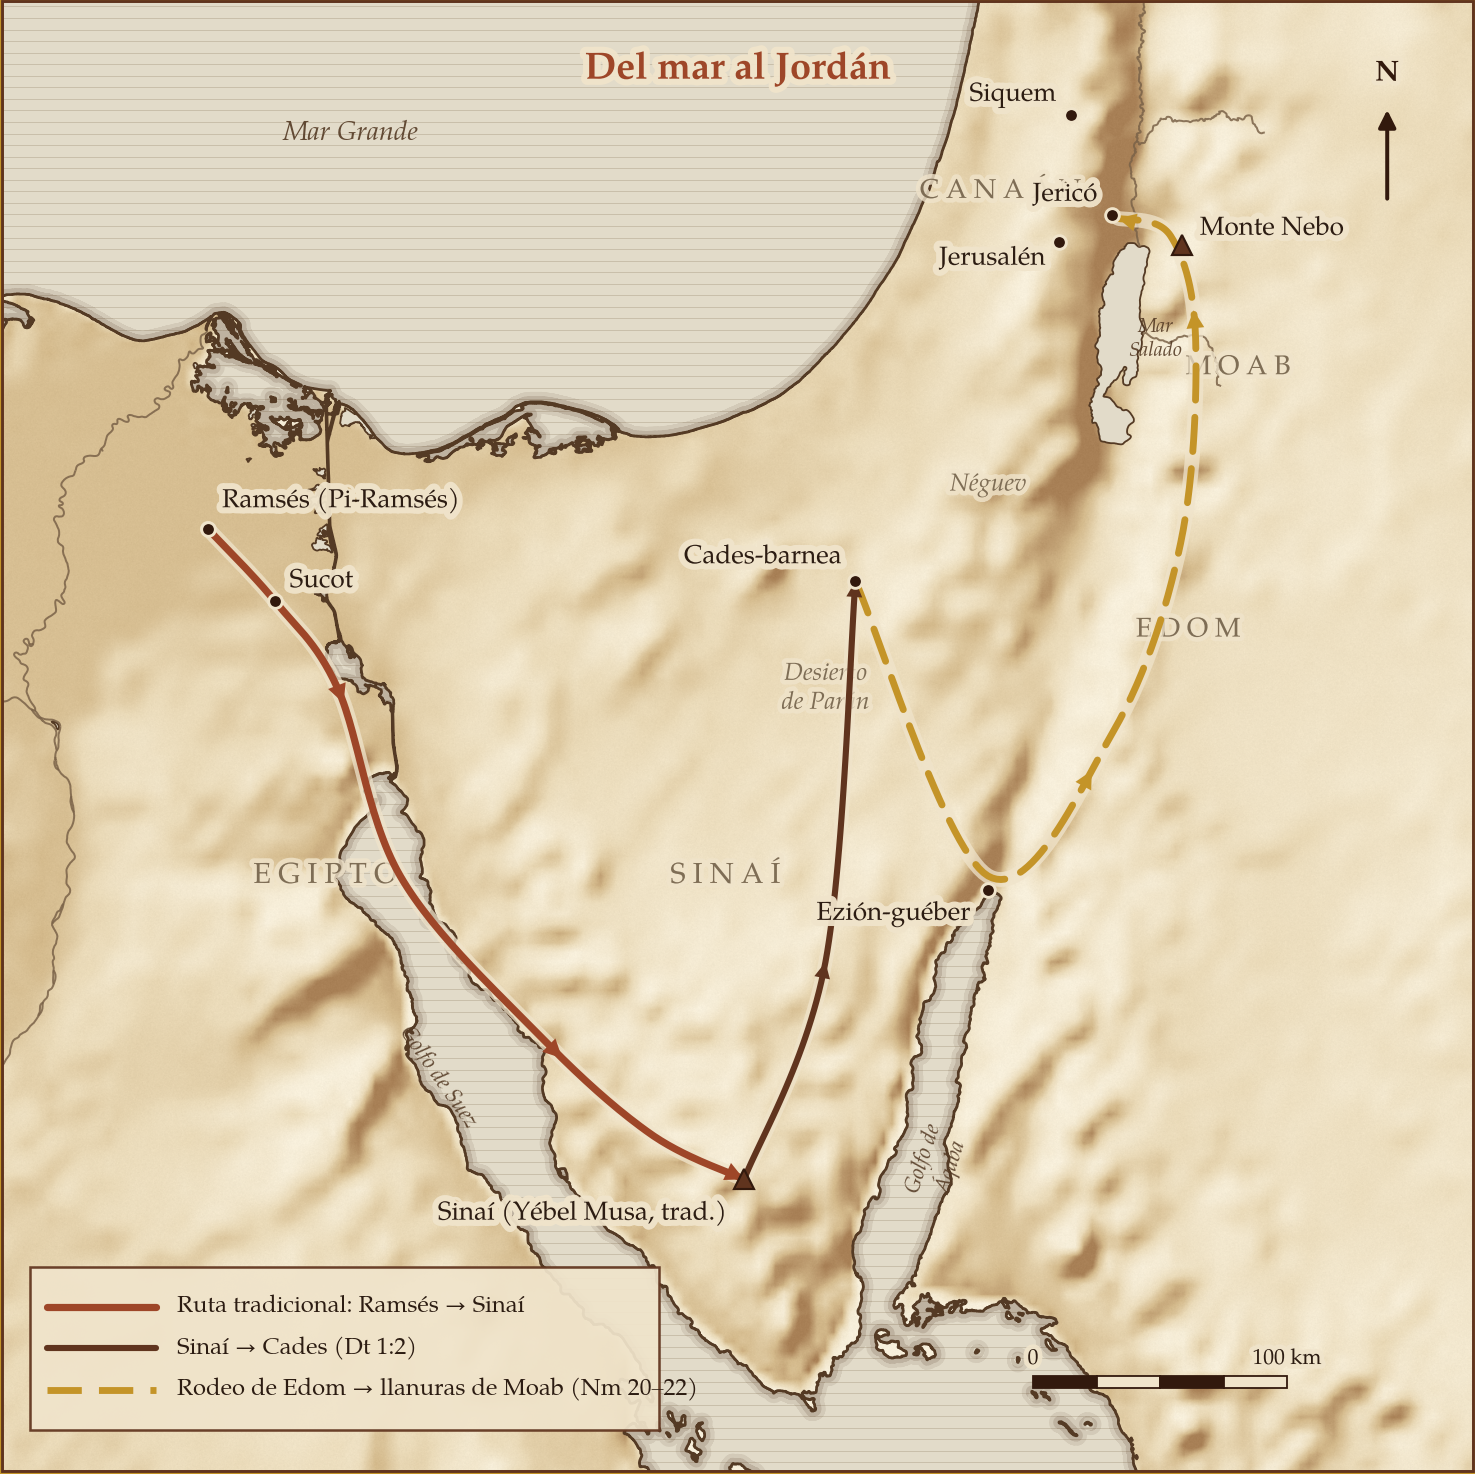
\includegraphics[width=0.97\linewidth]{mapa_exodo.png}
\end{minipage}\hspace{1.5em}
\begin{minipage}[b]{0.245\linewidth}\centering
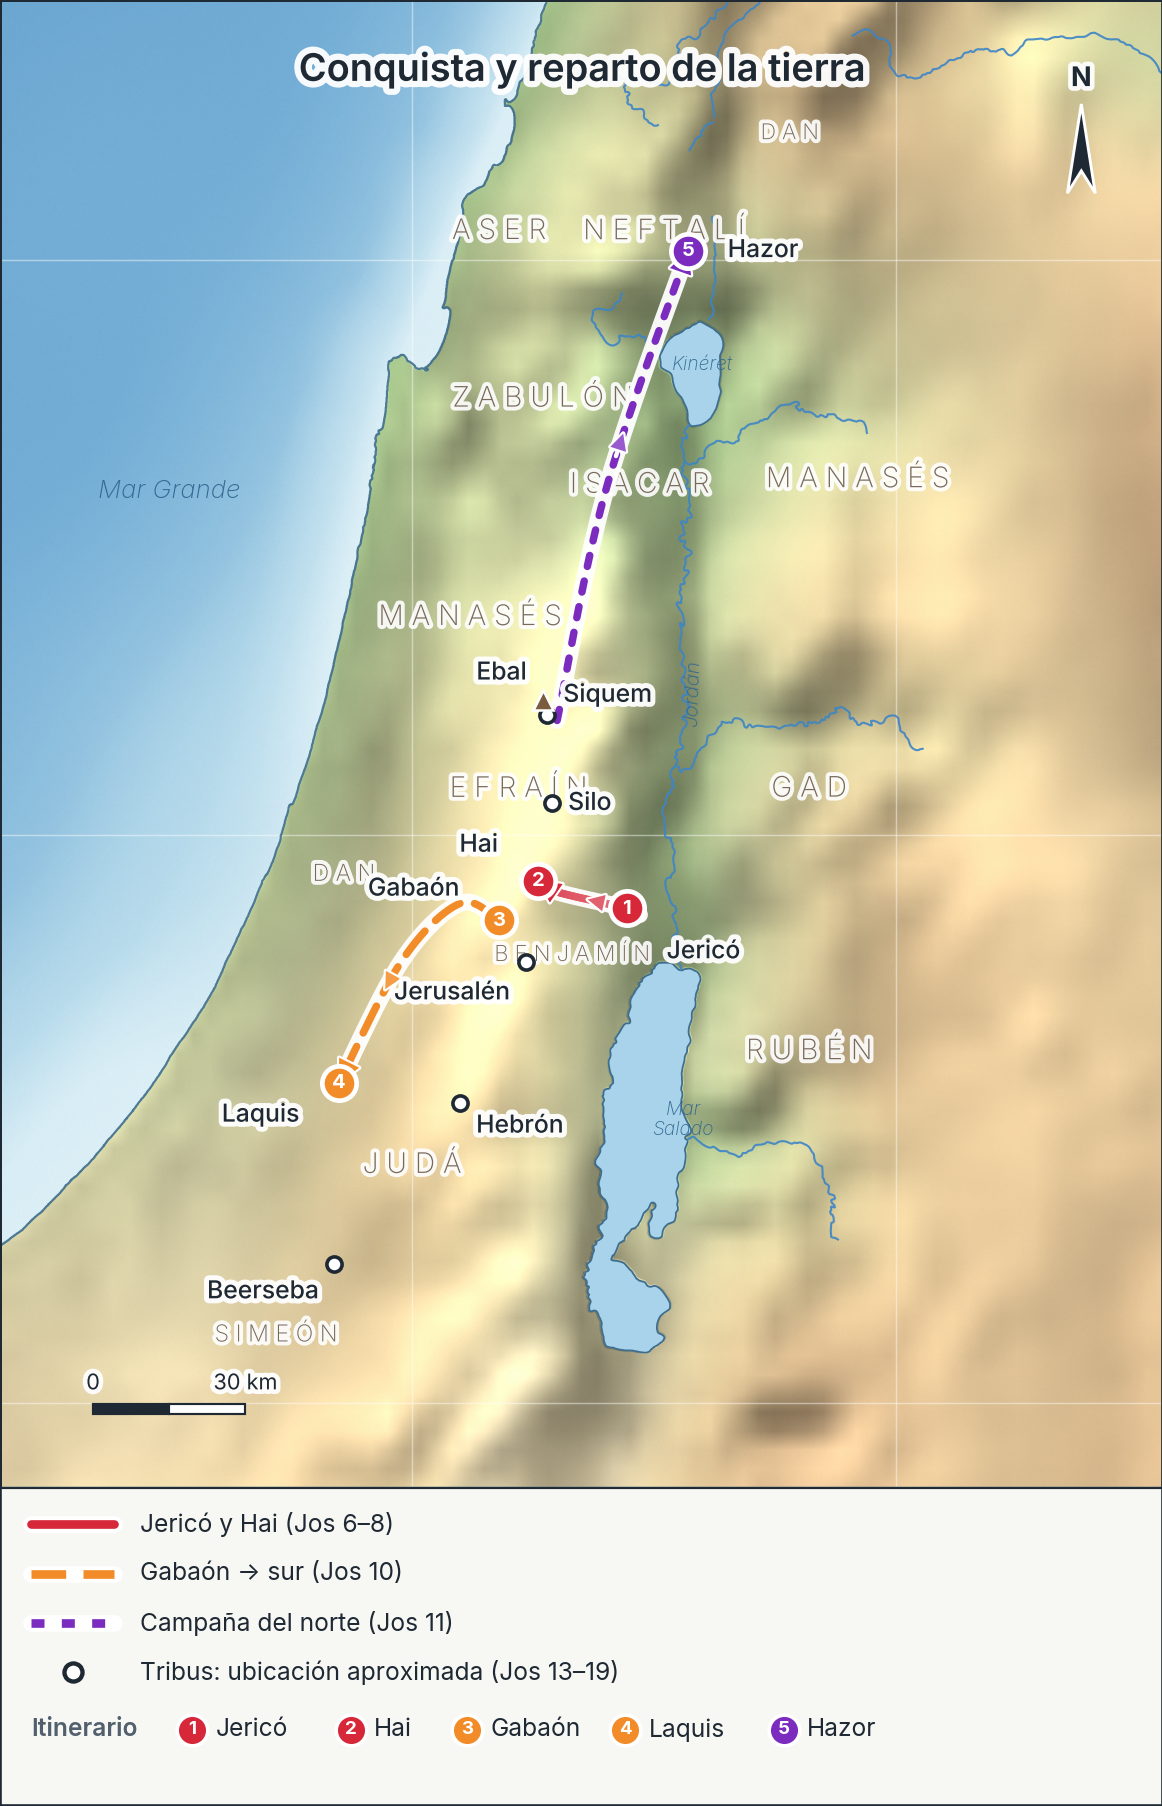
\includegraphics[width=0.97\linewidth]{mapa_tribus.png}
\end{minipage}\\[2pt]
{\footnotesize\color{sepia}\textit{Nota.} Elaboración propia: costas, lagos y ríos GSHHS/WDB y relieve sombreado (Basemap); ubicaciones antiguas aproximadas. Izquierda: ruta tradicional; el lugar del paso y del Sinaí está en debate. Derecha: tribus, ubicación aproximada.}
\end{center}

El mar del Éxodo es en hebreo \heb{יַם־סוּף} (\emph{yam suf}), «mar de los juncos», que la LXX tradujo «mar Rojo». Hoffmeier (2005) sitúa el paso en los lagos del istmo de Suez; Batto (1984), en el mar Rojo y sus golfos. El pacto sinaítico, en cambio, sigue el molde de los tratados hititas de vasallaje (Mendenhall, 1954), aunque Weinfeld (1972) halló paralelos de Dt 28 con tratados asirios del siglo \textsc{vii} y la fecha de redacción sigue discutida. En Tell Deir Alla, una inscripción del siglo \textsc{viii} a.\,e.\,c. comienza: «Escrito de Balaam, hijo de Beor, el que veía a los dioses» (Hoftijzer y van der Kooij, 1976); no confirma Nm 22–24, pero atestigua al vidente en esa región.

La destrucción de Jericó se ha fechado hacia 1400 a.\,e.\,c. (Garstang y Garstang, 1940; Wood, 1990) y hacia 1550 (Kenyon, 1957), y el radiocarbono dio fechas del siglo \textsc{xvi} (Bruins y van der Plicht, 1995). Hai (\heb{הָעַי}, «la ruina») suele identificarse con et-Tell, deshabitado en el Bronce Tardío (Callaway, 1968). Hazor sufrió en el siglo \textsc{xiii} una destrucción por fuego que Ben-Tor atribuye a Israel (Ben-Tor y Rubiato, 1999) y otros a una revuelta interna (Zuckerman, 2007). En el monte Ebal, Zertal (1985) interpretó una estructura del Hierro~I como el altar de Jos 8:30–35, y Kempinski (1986) como torre de vigilancia; la tablilla de plomo publicada en 2023 con una supuesta maldición en nombre de YHW (Stripling et al., 2023) ha sido muy cuestionada y no debe usarse como prueba. Las aldeas del Hierro~I en la sierra central, casi sin huesos de cerdo (Finkelstein, 1988), se leen como marcadores de una identidad nueva (Faust, 2006), y el libro de Josué narra la destrucción de solo tres ciudades seguida de un asentamiento prolongado (Kitchen, 2003). Lo que queda fuera del alcance de la arqueología es la memoria que define a Israel en todas sus fuentes: haber salido de Egipto y haber recibido la tierra como don.

\section{Desarrollo bíblico}

\subsection{Redimidos para ser reino de sacerdotes}
La primera ley que Israel recibe como pueblo es un calendario, y la sangre del cordero hace que el destructor «pase de largo» (\heb{פָּסַח}, \emph{pasaj}, Éx 12:13). El cántico del mar ya mira hacia adelante: Dios guía «en su misericordia» (\heb{בְחַסְדְּךָ}) al pueblo que «redimió» y lo plantará «en el monte de tu heredad» (15:13, 17). En el Sinaí, Dios habla antes de dar mandamiento alguno:

\begin{cita}Vosotros visteis lo que hice a los egipcios, y cómo os tomé sobre alas de águila y os he traído a mí. Ahora, pues, si de veras escucháis mi voz y guardáis mi pacto, seréis mi tesoro especial entre todos los pueblos, porque mía es toda la tierra. Y vosotros me seréis un reino de sacerdotes y una nación santa.\fuente{(Éx 19:4--6)}\end{cita}

La meta del Éxodo no era el Sinaí ni Canaán, sino «a mí». La condición, \heb{אִם־שָׁמוֹעַ תִּשְׁמְעוּ} (\emph{im shamoa tishmeú}), llega después, y por eso el pacto no crea la relación, que ya existe gracias a la redención, sino que define cómo se vive. \heb{סְגֻלָּה} (\emph{segulá}) es el tesoro personal de un rey (1~Cr 29:3; Sarna, 1991), y la frase «mía es toda la tierra» impide leerlo como desprecio de las naciones. \heb{מַמְלֶכֶת כֹּהֲנִים} (\emph{mamléjet kohaním}) pone a Israel ante los pueblos en el lugar que el sacerdote ocupa dentro de Israel, y \heb{גּוֹי קָדוֹשׁ} (\emph{goy qadosh}) le da el nombre común de las naciones, \emph{goy}, aunque apartada para Dios. Pedro cita la fórmula según la LXX para creyentes de Asia Menor (1~P 2:9), y amplía así la vocación de Israel sin traspasarla a otro pueblo, la lógica del olivo de Ro 11:17–24.

El Decálogo comienza con un indicativo, «yo soy YHWH tu Dios, que te saqué de la tierra de Egipto» (Éx 20:2), y la ley queda como forma de vida de un pueblo liberado, no como precio de su libertad. El pueblo responde «haremos y obedeceremos» (\heb{נַעֲשֶׂה וְנִשְׁמָע}, 24:7). La elección no se funda en mérito, sino en que «YHWH os amó y quiso guardar el juramento que juró a vuestros padres» (Dt 7:8), fundamento que Pablo invoca en Ro 11:28. El santuario tiene un propósito declarado, «habitaré en medio de ellos» (\heb{וְשָׁכַנְתִּי בְּתוֹכָם}, Éx 25:8). De \emph{shajan}, «habitar como en tienda», vienen \emph{mishkán} y el término rabínico \emph{Shejiná}. Al terminarse la obra, «la gloria de YHWH llenó el tabernáculo» (Éx 40:34), y muchos ven en ella «la gloria» de Ro 9:4 (Moo, 1996). El fin de la mediación sacerdotal lo expresa la bendición de Nm 6:24–27, conservada en dos rollitos de plata de Ketef Hinom (siglos \textsc{vii}–\textsc{vi} a.\,e.\,c.), los textos bíblicos más antiguos conocidos (Barkay et al., 2004).

\subsection{Ruptura y misericordia: el becerro y Cades}
Apenas cuarenta días después de «haremos y obedeceremos», el pueblo adora un becerro de oro (Éx 32:4), y Dios propone destruirlo y hacer de Moisés una gran nación (32:10), lo que equivalía a empezar de nuevo con otro Abraham. El argumento decisivo de la intercesión es el juramento: «acuérdate de Abraham, de Isaac y de Israel tus siervos, a los cuales has jurado por ti mismo» (32:13). El pacto con los padres, estudiado en el Estudio~1, se vuelve aquí por primera vez fundamento de una restauración. Moisés llega a ofrecer su vida, «ráeme ahora de tu libro» (32:32), como Pablo al abrir Romanos 9–11 (Ro 9:3; Moo, 1996). Entonces Dios revela su nombre:

\hebverso{יְהוָה יְהוָה אֵל רַחוּם וְחַנּוּן אֶרֶךְ אַפַּיִם וְרַב־חֶסֶד וֶאֱמֶת}
\begin{cita}¡YHWH, YHWH, Dios compasivo y clemente, lento para la ira y grande en misericordia y fidelidad; que guarda misericordia a millares, que perdona la iniquidad, la rebelión y el pecado, pero que de ningún modo tendrá por inocente al culpable!\fuente{(Éx 34:6--7)}\end{cita}

Ningún texto de restauración se cita tanto en la Biblia hebrea (Nm 14:18; Sal 103:8; Jl 2:13; Jon 4:2), y se pronuncia justo después de la ruptura. En su centro está \heb{חֶסֶד} (\emph{jésed}), la lealtad amorosa del pacto, y \heb{רַחוּם} (\emph{rajum}) viene de \emph{rejem}, «seno materno». El perdón no anula la justicia, aunque la misericordia «a millares» desborda la visitación «hasta la tercera y cuarta generación», y Dios escribe de nuevo las tablas (Éx 34:1, 27–28).

En Cades, tras el informe de los espías, el pueblo propone volver a Egipto (Nm 14:4), es decir, deshacer el Éxodo. Moisés intercede citando literalmente Éx 34:6–7 (Nm 14:17–19), y la respuesta tiene dos partes inseparables: \heb{סָלַחְתִּי כִּדְבָרֶךָ}, «lo he perdonado conforme a tu palabra» (14:20), pero esa generación morirá en el desierto y entrarán sus hijos, con Josué y Caleb (14:22–24, 31). Perdón para el pueblo, juicio sobre una generación y un remanente fiel: es la secuencia que Pablo reconocerá en su tiempo al hablar de «un remanente escogido por gracia» (Ro 11:5).

\subsection{En las llanuras de Moab}
Balaam, contratado para maldecir, solo consigue bendecir a Israel y anunciar que «saldrá una estrella de Jacob» (Nm 24:17), que el Targum Onqelos leyó como mesiánico. En Sitim, sin embargo, el pueblo se une al culto de Baal-peor (Nm 25:1–3), el primer caso de idolatría ligado a los cultos de la tierra y a la unión con otros pueblos, que los profetas recordarán como un quiebre (Os 9:10). Deuteronomio recoge después los discursos de Moisés a la generación nacida en el desierto, en torno al Shemá (Dt 6:4), y en ese umbral de la tierra anuncia con mayor claridad que ningún otro libro el destierro y el regreso, que se examinan en la sección~\ref{sec:resto}.

\subsection{Josué: la entrada en la tierra}
El cruce del Jordán reproduce el paso del mar, y la primera persona de Canaán que confiesa al Dios de Israel es Rahab: «YHWH vuestro Dios es Dios arriba en los cielos y abajo en la tierra» (Jos 2:11). Ella y su familia habitan «en medio de Israel hasta hoy» (6:25), y Mateo la incluye en la genealogía del Mesías (Mt 1:5). El caso muestra que el \heb{חֵרֶם} (\emph{jérem}), la «consagración al exterminio» (Jos 6:17), no se definía por la etnia. La Estela de Mesa usa la misma raíz, y los relatos de conquista antiguos emplean fórmulas hiperbólicas de destrucción total (Younger, 1990). La primera derrota, ante Hai, se debe a que Acán tomó parte del botín consagrado, y su castigo se ejecuta en el \heb{עֵמֶק עָכוֹר} (\emph{émeq Ajor}), «valle de la desgracia» (Jos 7:26), nombre al que Oseas volverá para anunciar la restauración.

El reparto termina con un balance: «no faltó palabra de todas las buenas promesas que YHWH había hecho a la casa de Israel; todo se cumplió» (Jos 21:45). La promesa a Abraham alcanza así un primer cumplimiento, aunque «queda aún mucha tierra por poseer» (Jos 13:1). En Siquem, donde Abraham recibió esa promesa, Josué llama a elegir, «yo y mi casa serviremos a YHWH» (24:15), el pueblo renueva el pacto y los huesos de José, traídos desde Egipto, reciben sepultura (24:32). El juramento de Gn 50:25 se cumple en el último versículo de la etapa.

\section{Israel como nación santa y reino de sacerdotes}

La fórmula de Éx 19:6 describe un llamado, no un logro. Israel lo vivió cuando dijo «haremos y obedeceremos» y la gloria llenó el tabernáculo; lo quebró al pie del monte, en Cades, en Baal-peor y con el robo de Acán; y en cada caso el llamado sobrevivió gracias a una mediación, la de Moisés, la de Finees, que recibió «el pacto de un sacerdocio perpetuo» (Nm 25:13), o la del remanente de Josué y Caleb. La vocación miraba además hacia las naciones, pues la Torá sería «sabiduría [\ldots] ante los ojos de los pueblos» (Dt 4:6) y Rahab fue incorporada. La santidad de Israel descansaba en la presencia de Dios más que en la perfección del pueblo, como Moisés reconoce: «¿en qué se conocerá que he hallado gracia ante tus ojos, yo y tu pueblo, sino en que tú andes con nosotros?» (Éx 33:16).

\section{Aporte de la tradición judía}

La memoria de esta etapa pervive en el calendario y la liturgia, que pertenecen a la tradición y no al texto bíblico. Shavuot, que la Torá presenta como fiesta de las primicias (Lv 23:15–21), es para la liturgia el «tiempo de la entrega de nuestra Torá», y el Talmud enseña que «cada palabra que salía de la boca del Todopoderoso se dividía en setenta lenguas» (Shabat 88b; Epstein, 1935–1948), el número tradicional de las naciones.

También las rupturas tienen su fecha. La Mishná enseña que el 17 de Tamuz se rompieron las tablas y que el 9 de Av «se decretó contra nuestros padres que no entrarían en la tierra», día en que cayeron además el primer y el segundo templo (Taanit 4:6; Danby, 1933). El Talmud lo explica con una palabra a la generación que lloró sin causa tras el informe de los espías: «vosotros llorasteis por nada; yo os estableceré un llanto por generaciones» (Taanit 29a). La tradición enlaza así Cades con las dos destrucciones de los estudios~5 y~7, pero el ayuno no tiene la última palabra. Según la cronología rabínica, Moisés descendió con las segundas tablas el 10 de Tishré, que quedó como Yom Kipur (Seder Olam 6; Guggenheimer, 1998), y en ese día y en las \emph{selijot} se recitan las \heb{שְׁלֹשׁ עֶשְׂרֵה מִדּוֹת} (\emph{shelosh esré midot}, «trece atributos») de Éx 34:6–7. El Talmud dice que Dios «mostró a Moisés el orden de la plegaria: siempre que Israel peque, que hagan delante de mí según este orden, y yo los perdonaré» (Rosh Hashaná 17b). La revelación que siguió al becerro se volvió así oración permanente de restauración.

\section{La promesa de restauración}\label{sec:resto}

En esta etapa la promesa es a la vez respuesta inmediata a la infidelidad (Éx 34; Nm 14) y profecía de un futuro lejano (Dt 4; 30; 32).

\begin{center}\small
\renewcommand{\arraystretch}{1.2}
\begin{tabular}{>{\RaggedRight\arraybackslash}p{2.5cm}>{\RaggedRight\arraybackslash}p{5.4cm}>{\RaggedRight\arraybackslash}p{6.0cm}}
\toprule
\textbf{Texto} & \textbf{Promesa} & \textbf{Proyección}\\
\midrule
Éx 32:13; 34:6–10 & Perdón fundado en el juramento a los padres y en el nombre misericordioso & Nm 14:18; Jl 2:13; Jon 4:2; Sal 103:8\\
Nm 14:20–24 & Perdón del pueblo, juicio de una generación, entrada del remanente & Is 10:20–22; Ro 9:27; 11:5\\
Dt 4:25–31 & Destierro anunciado; regreso «en los postreros días» & Os 3:5; Jer 29:12–14\\
Dt 30:1–10 & Regreso de la dispersión; corazón circuncidado & Jer 31:33 [31:32]; Ez 36:24–27; Ro 10:6–8\\
Dt 32:36–43 & Compasión de Dios; las naciones se alegran con su pueblo & Ro 10:19; 11:11; 15:10\\
\bottomrule
\end{tabular}\end{center}

Sin que Israel haya entrado aún en la tierra, Moisés anuncia que la perderá, «YHWH os esparcirá entre los pueblos» (Dt 4:27), y que el destierro no tendrá la última palabra:

\hebverso{בַּצַּר לְךָ וּמְצָאוּךָ כֹּל הַדְּבָרִים הָאֵלֶּה בְּאַחֲרִית הַיָּמִים וְשַׁבְתָּ עַד־יְהוָה אֱלֹהֶיךָ וְשָׁמַעְתָּ בְּקֹלוֹ\\
כִּי אֵל רַחוּם יְהוָה אֱלֹהֶיךָ לֹא יַרְפְּךָ וְלֹא יַשְׁחִיתֶךָ וְלֹא יִשְׁכַּח אֶת־בְּרִית אֲבֹתֶיךָ אֲשֶׁר נִשְׁבַּע לָהֶם}
\begin{cita}Cuando estés en angustia y te alcancen todas estas cosas, en los postreros días, volverás a YHWH tu Dios y escucharás su voz. Porque Dios compasivo es YHWH tu Dios; no te dejará, ni te destruirá, ni se olvidará del pacto que juró a tus padres.\fuente{(Dt 4:30--31)}\end{cita}

De aquí tomarán los profetas la expresión \heb{בְּאַחֲרִית הַיָּמִים} (\emph{be-ajarit ha-yamim}, «en los postreros días»), el verbo \emph{shuv} («volverás») y el \emph{rajum} de Éx 34:6. El regreso descansa, pues, sobre el carácter de Dios revelado tras el becerro y sobre el juramento a los padres, y ONE FOR ISRAEL (2025) cuenta este pasaje entre los que anuncian el regreso de Israel a Dios que Pablo espera en Ro 11:26. Dt 30 lo desarrolla: Israel «volverá» (v. 2), Dios «hará volver tu cautividad» (\heb{אֶת־שְׁבוּתְךָ}, \emph{et shevutejá}, v. 3), lo recogerá aunque esté «en el extremo de los cielos» (v. 4) y hará lo que Israel no puede hacer:

\hebverso{וּמָל יְהוָה אֱלֹהֶיךָ אֶת־לְבָבְךָ וְאֶת־לְבַב זַרְעֶךָ לְאַהֲבָה אֶת־יְהוָה אֱלֹהֶיךָ בְּכָל־לְבָבְךָ וּבְכָל־נַפְשְׁךָ לְמַעַן חַיֶּיךָ}
\begin{cita}Y circuncidará YHWH tu Dios tu corazón y el corazón de tu descendencia, para que ames a YHWH tu Dios con todo tu corazón y con toda tu alma, a fin de que vivas.\fuente{(Dt 30:6)}\end{cita}

Lo que en Dt 10:16 era mandato se ha vuelto promesa: que Israel pueda por fin cumplir el Shemá. El Cántico de Moisés añade el resto del arco. Tras la infidelidad y el juicio, «YHWH juzgará a su pueblo, y por amor de sus siervos se arrepentirá» (Dt 32:36); antes, Dios ha respondido a la idolatría con una paradoja, «yo también los provocaré a celos con un pueblo que no es pueblo» (\heb{וַאֲנִי אַקְנִיאֵם בְּלֹא־עָם}, 32:21), y el cántico se cierra llamando a las naciones a alegrarse con Israel (32:43), en la forma más larga que conservan 4QDeut\textsuperscript{q} y la LXX, \grc{εὐφράνθητε, ἔθνη, μετὰ τοῦ λαοῦ αὐτοῦ} (Tov, 2012).

Los profetas leen el futuro con estas mismas imágenes. Isaías promete que «habrá camino para el remanente de su pueblo, como lo hubo para Israel el día que subió de la tierra de Egipto» (Is 11:16), y que Éx 19:6 se cumplirá en Sion (Is 61:6). Jeremías, que llama a Israel «primicias» de YHWH (Jer 2:3; cf. Ro 11:16), responde a la ruptura del Sinaí con un pacto nuevo:

\hebverso{הִנֵּה יָמִים בָּאִים נְאֻם־יְהוָה וְכָרַתִּי אֶת־בֵּית יִשְׂרָאֵל וְאֶת־בֵּית יְהוּדָה בְּרִית חֲדָשָׁה}
\begin{cita}He aquí que vienen días, dice YHWH, en que haré un nuevo pacto con la casa de Israel y con la casa de Judá. [\ldots] Pondré mi ley en su interior y la escribiré en su corazón [\ldots], porque perdonaré su maldad y no me acordaré más de su pecado.\fuente{(Jer 31:31--34 [31:30--33])}\end{cita}

La ley sigue siendo «mi ley»; lo que cambia es el lugar donde se escribe, que pasa de la piedra al corazón, como había prometido Dt 30:6. Tampoco cambian los destinatarios, «la casa de Israel y la casa de Judá», es decir, el reino del norte, ya deportado por Asiria cuando escribe Jeremías, y el reino del sur, distinción que se tratará en los estudios~4 y~5. El perdón final es el de Éx 34:6–7, y con esa idea cerrará Pablo su argumento: «este será mi pacto con ellos, cuando yo quite sus pecados» (Ro 11:27). Oseas, por su parte, vuelve al lugar del pecado de Acán y anuncia que Dios dará a Israel «el valle de Acor por puerta de esperanza; y allí responderá como en los días de su juventud, como en el día en que subió de la tierra de Egipto» (Os 2:15 [2:17]). Por donde Israel cayó al comenzar la conquista volverá a entrar, y el «no sois mi pueblo» de Os 1:9 se convertirá en «sois hijos del Dios viviente» (1:10 [2:1]), textos que Pablo cita en Ro 9:25–26.

Ninguna etapa aporta a Romanos 9–11 tantos textos como esta. En Ro 10:6–8 identifica la palabra cercana de Dt 30:12–14, prometida para el tiempo del regreso, con «la palabra de fe que predicamos». Con Dt 32:21 explica que «por su transgresión vino la salvación a los gentiles, para provocarles a celos» (\grc{εἰς τὸ παραζηλῶσαι αὐτούς}, Ro 11:11): los celos del Cántico son el medio por el que Dios atraerá de nuevo a Israel. En Ro 11:8 une Dt 29:4 [29:3] con Is 29:10, «ojos con que no vean y oídos con que no oigan, hasta el día de hoy», y sitúa el endurecimiento de su tiempo en el mismo arco que en Deuteronomio va de la ceguera a la circuncisión del corazón. Al decir a gentiles que «nuestros padres» pasaron el mar (1~Co 10:1), pone a la iglesia dentro del relato del Éxodo, no en su lugar (Hays, 1989). Lo que Moisés anunció para «los postreros días» es, en suma, lo que Pablo espera cuando afirma que «todo Israel será salvo» (Ro 11:26), tema del Estudio~8.

\section{Conclusión y puente al Estudio 3}

Entre el Éxodo y la muerte de Josué toma forma la vocación que el Estudio~1 había dejado en germen. Dios redime antes de legislar, y en el Sinaí Israel recibe su identidad de \emph{segulá}, \emph{mamléjet kohaním} y \emph{goy qadosh}, con Dios habitando en medio de él. La vocación se quiebra casi en el acto, y Dios responde con perdón, mediador y remanente. Lo decisivo para esta serie es que la restauración ya está escrita en la Torá: antes de que Israel entre en la tierra, Deuteronomio anuncia el destierro, el regreso y un corazón circuncidado, y el Cántico prevé los celos y la alegría común de las naciones con Israel. Isaías, Jeremías y Oseas leerán el futuro como un nuevo éxodo y un nuevo pacto, y Pablo construirá Romanos 9–11 con esos mismos textos, convencido de que el llamamiento recibido en el Sinaí no ha sido revocado.

La tierra había sido dada, pero el libro de los Jueces se abre con una advertencia: «se levantó después de ellos otra generación que no conocía a YHWH, ni la obra que él había hecho por Israel» (Jue 2:10). Esa generación olvidará el Éxodo y comenzará un ciclo de apostasía, opresión, clamor y liberación, en el que surgirán Rut, una moabita incorporada a Israel, y Samuel, que ungirá a Saúl y a David. De ello se ocupa el Estudio~3: \emph{de los Jueces a David}.

\section*{Preguntas para la reflexión}\markboth{Preguntas para la reflexión}{}
\begin{enumerate}
\item Dios dice «os he traído a mí» (Éx 19:4) antes de dar un solo mandamiento. ¿Qué cambia en la manera de entender la ley cuando se lee después de la redención?
\item Dios revela su nombre misericordioso (Éx 34:6–7) justo después del becerro de oro. ¿Qué enseña este orden sobre la relación entre el pecado de Israel y la fidelidad de Dios en Romanos 11?
\item Pablo dice a creyentes gentiles que «nuestros padres» pasaron el mar (1~Co 10:1). ¿Qué implica recibir como propia la historia de Israel, y qué responsabilidad trae (Ro 11:18–21)?
\end{enumerate}

\section*{Glosario}\markboth{Glosario}{}
\begin{description}\small
\item[Émeq Ajor] (\heb{עֵמֶק עָכוֹר}). «Valle de la desgracia», lugar del castigo de Acán (Jos 7:26); «puerta de esperanza» en Os 2:15 [2:17].
\item[Jésed] (\heb{חֶסֶד}). Lealtad amorosa propia del pacto; centro de Éx 34:6–7.
\item[Mamléjet kohaním] (\heb{מַמְלֶכֶת כֹּהֲנִים}). «Reino de sacerdotes» (Éx 19:6); LXX \grc{βασίλειον ἱεράτευμα}.
\item[Mishkán] (\heb{מִשְׁכָּן}). Tabernáculo, «morada», de \emph{shajan}, «habitar» (Éx 25:9; 40:34).
\item[Segulá] (\heb{סְגֻלָּה}). Tesoro personal de un rey; Israel como propiedad especial de Dios (Éx 19:5; Dt 7:6; Mal 3:17).
\item[Shelosh esré midot] (\heb{שְׁלֹשׁ עֶשְׂרֵה מִדּוֹת}). «Trece atributos» de Dios según la división rabínica de Éx 34:6–7.
\end{description}

\section*{Referencias}\markboth{Referencias}{}
{\small
\refapa{Barkay, G., Vaughn, A.~G., Lundberg, M.~J., \& Zuckerman, B. (2004). The amulets from Ketef Hinnom: A new edition and evaluation. \emph{Bulletin of the American Schools of Oriental Research, 334}, 41--71.}
\refapa{Batto, B.~F. (1984). The Reed Sea: Requiescat in pace. \emph{Journal of Biblical Literature, 103}(1), 27--35.}
\refapa{Ben-Tor, A., \& Rubiato, M.~T. (1999). Excavating Hazor, part two: Did the Israelites destroy the Canaanite city? \emph{Biblical Archaeology Review, 25}(3).}
\refapa{\emph{Biblia Hebraica Stuttgartensia} (5.ª ed.). (1997). Deutsche Bibelgesellschaft.}
\refapa{Bimson, J.~J. (1978). \emph{Redating the Exodus and conquest}. JSOT Press.}
\refapa{Bruins, H.~J., \& van der Plicht, J. (1995). Tell es-Sultan (Jericho): Radiocarbon results of short-lived cereal and multiyear charcoal samples from the end of the Middle Bronze Age. \emph{Radiocarbon, 37}(2), 213--220.}
\refapa{Callaway, J.~A. (1968). New evidence on the conquest of `Ai. \emph{Journal of Biblical Literature, 87}(3), 312--320.}
\refapa{Danby, H. (Trad.). (1933). \emph{The Mishnah}. Oxford University Press.}
\refapa{Epstein, I. (Ed.). (1935--1948). \emph{The Babylonian Talmud}. Soncino Press.}
\refapa{Faust, A. (2006). \emph{Israel's ethnogenesis: Settlement, interaction, expansion and resistance}. Equinox.}
\refapa{Finkelstein, I. (1988). \emph{The archaeology of the Israelite settlement}. Israel Exploration Society.}
\refapa{Garstang, J., \& Garstang, J.~B.~E. (1940). \emph{The story of Jericho}. Hodder \& Stoughton.}
\refapa{Guggenheimer, H.~W. (1998). \emph{Seder Olam: The rabbinic view of biblical chronology}. Jason Aronson.}
\refapa{Hays, R.~B. (1989). \emph{Echoes of Scripture in the letters of Paul}. Yale University Press.}
\refapa{Hoffmeier, J.~K. (1997). \emph{Israel in Egypt: The evidence for the authenticity of the Exodus tradition}. Oxford University Press.}
\refapa{Hoffmeier, J.~K. (2005). \emph{Ancient Israel in Sinai: The evidence for the authenticity of the wilderness tradition}. Oxford University Press.}
\refapa{Hoftijzer, J., \& van der Kooij, G. (1976). \emph{Aramaic texts from Deir `Alla}. Brill.}
\refapa{Kempinski, A. (1986). Joshua's altar: An Iron Age I watchtower. \emph{Biblical Archaeology Review, 12}(1).}
\refapa{Kenyon, K.~M. (1957). \emph{Digging up Jericho}. Ernest Benn.}
\refapa{Kitchen, K.~A. (2003). \emph{On the reliability of the Old Testament}. Eerdmans.}
\refapa{Mendenhall, G.~E. (1954). Covenant forms in Israelite tradition. \emph{The Biblical Archaeologist, 17}(3), 50--76.}
\refapa{Moo, D.~J. (1996). \emph{The epistle to the Romans}. Eerdmans.}
\refapa{Moran, W.~L. (Ed. y Trad.). (1992). \emph{The Amarna letters}. Johns Hopkins University Press.}
\refapa{\emph{Novum Testamentum Graece} (28.ª ed.). (2012). Deutsche Bibelgesellschaft.}
\refapa{ONE FOR ISRAEL Ministry. (2025, 3 de julio). \emph{What does «all Israel will be saved» mean in Romans 11?} \url{https://www.oneforisrael.org/what-does-all-israel-will-be-saved-mean-in-romans-11/}}
\refapa{Rahlfs, A., \& Hanhart, R. (Eds.). (2006). \emph{Septuaginta} (ed. rev.). Deutsche Bibelgesellschaft.}
\refapa{Sarna, N.~M. (1991). \emph{Exodus} (The JPS Torah Commentary). Jewish Publication Society.}
\refapa{Stripling, S., Galil, G., Kumpova, I., Valach, J., et al. (2023). «You are cursed by the god YHW»: An early Hebrew inscription from Mt. Ebal. \emph{Heritage Science, 11}, 105.}
\refapa{Tov, E. (2012). \emph{Textual criticism of the Hebrew Bible} (3.ª ed.). Fortress Press.}
\refapa{Weinfeld, M. (1972). \emph{Deuteronomy and the Deuteronomic school}. Clarendon Press.}
\refapa{Wood, B.~G. (1990). Did the Israelites conquer Jericho? A new look at the archaeological evidence. \emph{Biblical Archaeology Review, 16}(2), 44--58.}
\refapa{Younger, K.~L., Jr. (1990). \emph{Ancient conquest accounts: A study in ancient Near Eastern and biblical history writing}. JSOT Press.}
\refapa{Zertal, A. (1985). Has Joshua's altar been found on Mt. Ebal? \emph{Biblical Archaeology Review, 11}(1), 26--43.}
\refapa{Zuckerman, S. (2007). Anatomy of a destruction: Crisis architecture, termination rituals and the fall of Canaanite Hazor. \emph{Journal of Mediterranean Archaeology, 20}(1), 3--32.}
}
\end{document}
